%%%%%%%%%%%%%%%%%%%%%%%%%%%%%%%%%%%%%%%%%
% Beamer Presentation
% LaTeX Template
% Version 1.0 (10/11/12)
%
% This template has been downloaded from:
% http://www.LaTeXTemplates.com
%
% License:
% CC BY-NC-SA 3.0 (http://creativecommons.org/licenses/by-nc-sa/3.0/)
%
%%%%%%%%%%%%%%%%%%%%%%%%%%%%%%%%%%%%%%%%%

%----------------------------------------------------------------------------------------
%	PACKAGES AND THEMES
%----------------------------------------------------------------------------------------
\documentclass{beamer}
\usepackage{amsmath, amsthm, amsfonts}
\usepackage{graphicx}
\usepackage{caption}
\usepackage{subcaption}
\usepackage[hyperref, UTF8]{ctex}

\mode<presentation> {

% The Beamer class comes with a number of default slide themes
% which change the colors and layouts of slides. Below this is a list
% of all the themes, uncomment each in turn to see what they look like.

%\usetheme{default}
%\usetheme{AnnArbor}
%\usetheme{Antibes}
%\usetheme{Bergen}
%\usetheme{Berkeley}
%\usetheme{Berlin}
%\usetheme{Boadilla}
%\usetheme{CambridgeUS}
%\usetheme{Copenhagen}
%\usetheme{Darmstadt}
%\usetheme{Dresden}
%\usetheme{Frankfurt}
%\usetheme{Goettingen}
%\usetheme{Hannover}
%\usetheme{Ilmenau}
%\usetheme{JuanLesPins}
%\usetheme{Luebeck}
\usetheme{Madrid}
%\usetheme{Malmoe}
%\usetheme{Marburg}
%\usetheme{Montpellier}
%\usetheme{PaloAlto}
%\usetheme{Pittsburgh}
%\usetheme{Rochester}
%\usetheme{Singapore}
%\usetheme{Szeged}
%\usetheme{Warsaw}

% As well as themes, the Beamer class has a number of color themes
% for any slide theme. Uncomment each of these in turn to see how it
% changes the colors of your current slide theme.

%\usecolortheme{albatross}
%\usecolortheme{beaver}
%\usecolortheme{beetle}
%\usecolortheme{crane}
%\usecolortheme{dolphin}
%\usecolortheme{dove}
%\usecolortheme{fly}
%\usecolortheme{lily}
%\usecolortheme{orchid}
%\usecolortheme{rose}
%\usecolortheme{seagull}
%\usecolortheme{seahorse}
%\usecolortheme{whale}
%\usecolortheme{wolverine}

%\setbeamertemplate{footline} % To remove the footer line in all slides uncomment this line
%\setbeamertemplate{footline}[page number] % To replace the footer line in all slides with a simple slide count uncomment this line

%\setbeamertemplate{navigation symbols}{} % To remove the navigation symbols from the bottom of all slides uncomment this line
}

\usepackage{graphicx} % Allows including images
\usepackage{booktabs} % Allows the use of \toprule, \midrule and \bottomrule in tables

%----------------------------------------------------------------------------------------
%	TITLE PAGE
%----------------------------------------------------------------------------------------

\title[Isotopic Approximation]{最近工作进展} % The short title appears at the bottom of every slide, the full title is only on the title page

\author{ 张胜威} % Your name
\institute[ZJU] % Your institution as it will appear on the bottom of every slide, may be shorthand to save space
{
ZJU\\ % Your institution for the title page
\medskip
%%\textit{john@smith.com} % Your email address
}
\date{\today} % Date, can be changed to a custom date

\begin{document}

\begin{frame}
\titlepage % Print the title page as the first slide
\end{frame}

\begin{frame}
\frametitle{背景} % Table of contents slide, comment this block out to remove it
\tableofcontents %Throughout your presentation, if you choose to use \section{} and \subsection{} commands, these will automatically be printed on this slide as an overview of your presentation
\begin{block}{目的}
为了方便模型的存储,传输和编辑等.在给定误差下,用一个尽可能粗糙的网格来近似原网格.
\end{block}
\begin{example}[目标]
  \begin{figure}[h]
    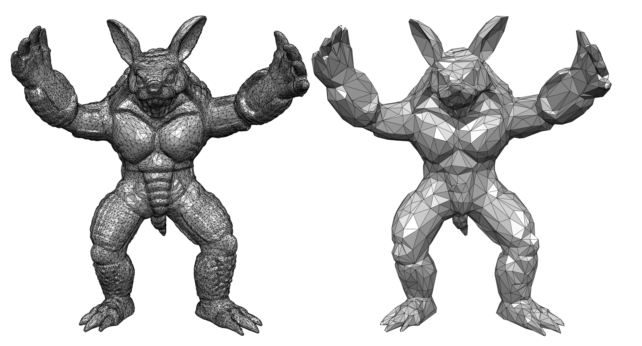
\includegraphics[width=6cm]{res}
  \end{figure}
\end{example}
\end{frame}


\begin{frame}
  \frametitle{论文的主要思想}
  \begin{itemize}
    \item 构造一个误差空间的体网格.
    \item 对于中间层zero\_surface做edge collapse, 保证collapse完了之后zero\_surface仍在误差空间体内部.
  \end{itemize}

  \begin{figure}[h]
    \begin{subfigure}[b]{0.4\textwidth}
      \includegraphics[width=\textwidth]{volume.png}
      \caption[a]{}
    \end{subfigure}
    \begin{subfigure}[b]{0.4\textwidth}
      \includegraphics[width=\textwidth]{volume2.png}
      \caption[b]{}
    \end{subfigure}
  \end{figure}
\end{frame}

\begin{frame}
  \frametitle{实现}
  \begin{block}{论文的实现}
    \begin{itemize}
      \item 构造误差空间体网格和zero\_surface(Refine).
      \item (通过控制函数f的error)做 zero\_surface的edge collapse.
    \end{itemize}
  \end{block}

  \begin{figure}
    \begin{subfigure}[b]{0.4\textwidth}
      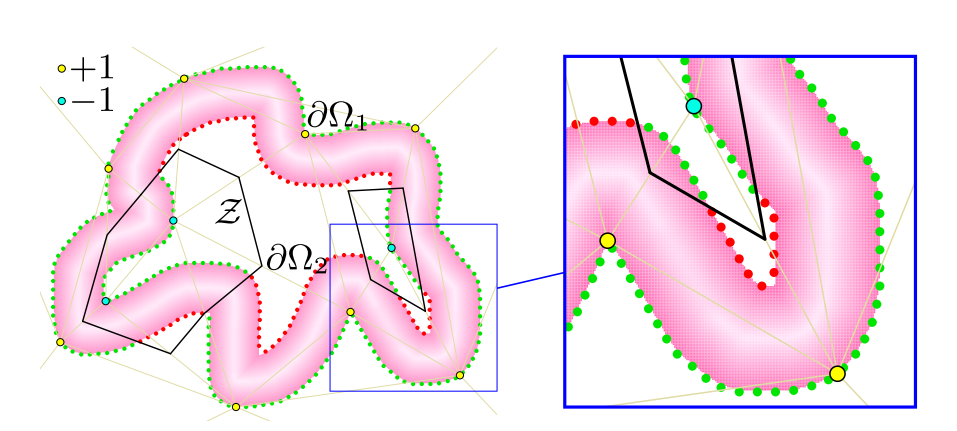
\includegraphics[width=\textwidth]{2.png}
      \caption[a]{构造误差空间体网格和zero\_surface,2D的示意图}
    \end{subfigure}
    \begin{subfigure}[b]{0.4\textwidth}
      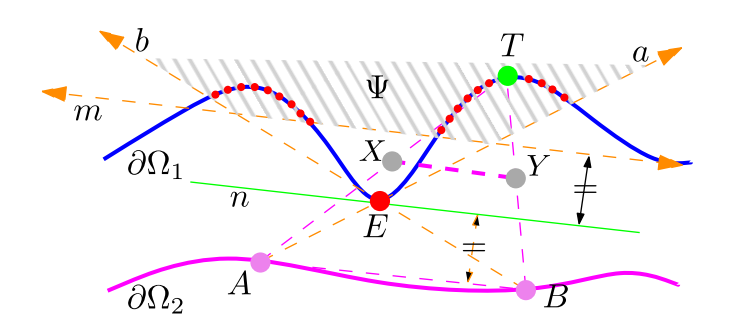
\includegraphics[width=\textwidth]{8.png}
      \caption[b]{误差控制}
    \end{subfigure}
  \end{figure}
\end{frame}

\begin{frame}{实现}
  \begin{block}{我现在的实现}
    \begin{itemize}
      \item 输入的bo+zero\_surface四面体化;bi+zero\_surface四面体化.两个做一个合并构成误差空间体网格.
      \item 在保证不与内外表面相交的情况下,直接对 zero\_surface做edge collapse.
    \end{itemize}
  \end{block}
\end{frame}

\begin{frame}
  \frametitle{进展}
  \begin{block}{构造误差空间体网格的策略}
    \begin{figure}
      \includegraphics[width=6cm]{teaport.png}
      \caption{外层的tetmesh(bo+zero\_surface的四面体化) 有自交}
    \end{figure}
  \end{block}
\end{frame}

\begin{frame}
  \frametitle{进展}
  \begin{block}{zero\_surface edge collapse}
    现在用Ipopt在这条边的一环邻域的kernel region中寻找合并点.这是一个强条件(能够保证新模型不会和内外表面相交).
    接下来将约束条件放松,只要不与内外表面相交即可.
  \end{block}
\end{frame}

\begin{frame}
  \frametitle{关于面试}
  \begin{block}{重要的几项}
    \begin{itemize}
      \item 基本的coding能力,写一手漂亮的代码.(正确,美观)
      \item 交流沟通(能够快速地理解所提的问题,描述清楚自己做的project)
    \end{itemize}
  \end{block}
\end{frame}

\begin{frame}%%[plain]

  \begin{columns}
    \begin{column}{\textwidth}
      \begin{center}
        \font\endfont = cmss10 at 25.40mm
        \endfont 
        \baselineskip 20.0mm
        Thank you!
      \end{center}    
    \end{column}
  \end{columns}
\end{frame}
%------------------------------------------------
%----------------------------------------------------------------------------------------

\end{document} 
